% !TeX root = ssre.tex
\section{Results}
Before any type of attack, the attacker is prompted by the program with the choice of the victims' IP - based on the ARP table - and the type of attack desired, based on FTP, SNMP, Telnet or SMTP . This workflow is shown in figure \ref{fig:WorkFlow}.

\begin{figure}[h!]
    \centering
    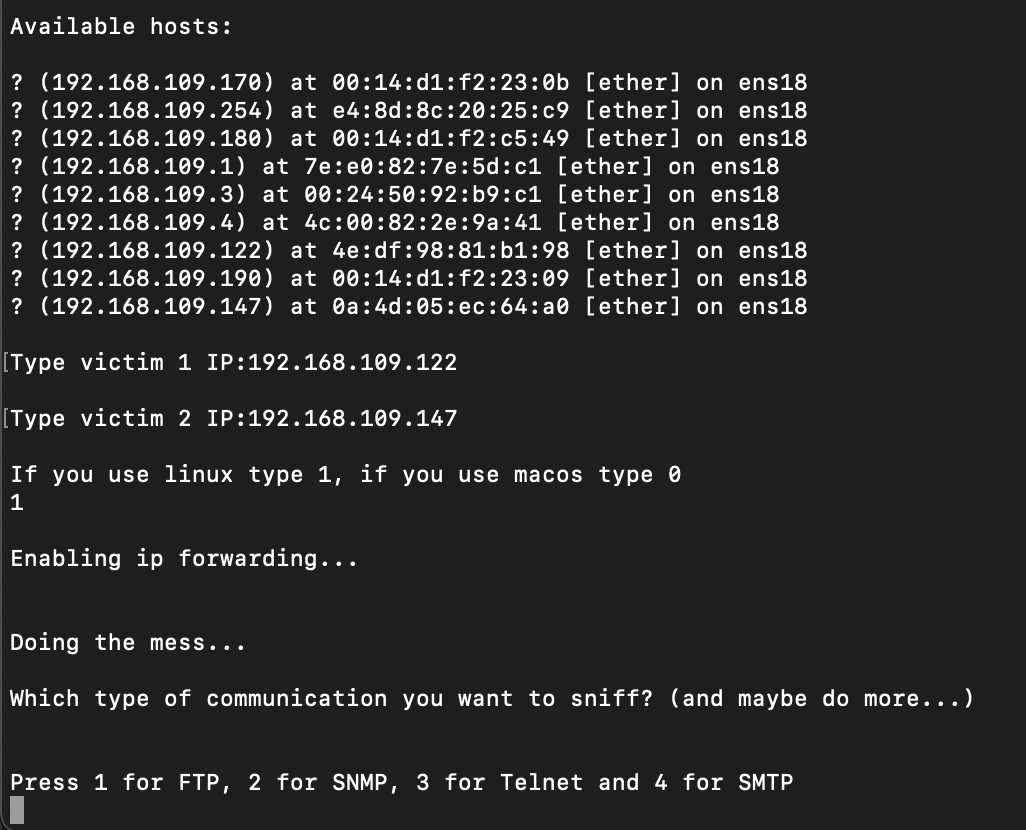
\includegraphics[width=0.85\linewidth,keepaspectratio]{Choice.png}
    \caption{Choice of victims and desired attack}
    \label{fig:WorkFlow}
\end{figure}
\FloatBarrier

The demonstration of the FTP passive attack was accomplished by creating a user and password associated to a FTP account that the FTP server recognizes as being valid. As depict in figure \ref{fig:FTPAttack}, one of the victims (\textit{192.168.109.122}) is accessing the FTP server located at \textit{192.168.109.147} and the attacker (left in the figure) has real-time access to the user and pass as valid credentials. 

\begin{figure}[h!]
    \centering
    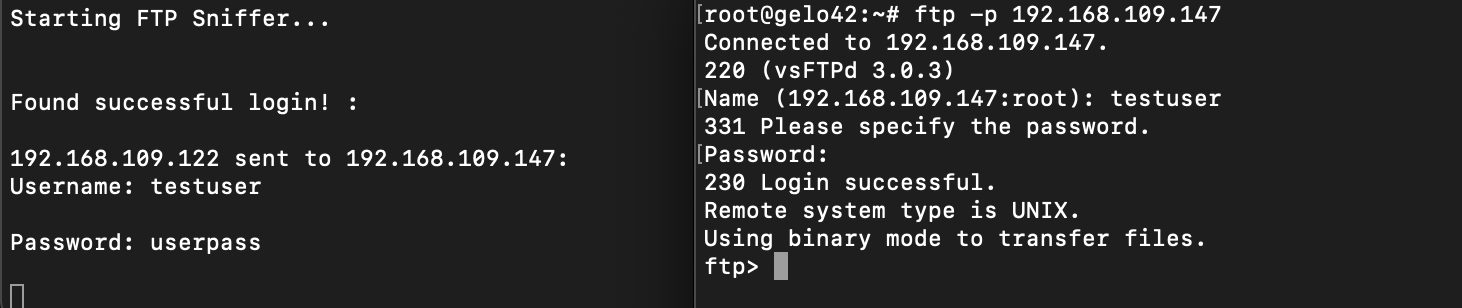
\includegraphics[width=1\linewidth,keepaspectratio]{FTPAttack.png}
    \caption{FTP passive attack}
    \label{fig:FTPAttack}
\end{figure}
\FloatBarrier

For the demonstration of both SNMP active and passive attack, the below described environment was created: 
\\\\
As shown in figure \ref{fig:SNMPPassiveAttack}, a remote user is querying the machine at \textit{192.168.109.147} about its System Up Time, using a \textit{snmpget} command. The attacker (left in the figure) is prompted with real-time data about the response to that command, including the community string \textit{veryprivate}. To perform the active attack, the user must type \textit{Ctrl-C} and enter, as described in section \ref{sec:Solution}, the necessary information. As depicted in figure \ref{fig:SNMPActiveAttack}, the victim of this attack in this created environment is running Debian with kernel version 4.19, it's a 64bit OS and the hostname is "gelo43". Those types of information can be useful for any other type of attacks. 

\begin{figure}[h!]
    \centering
    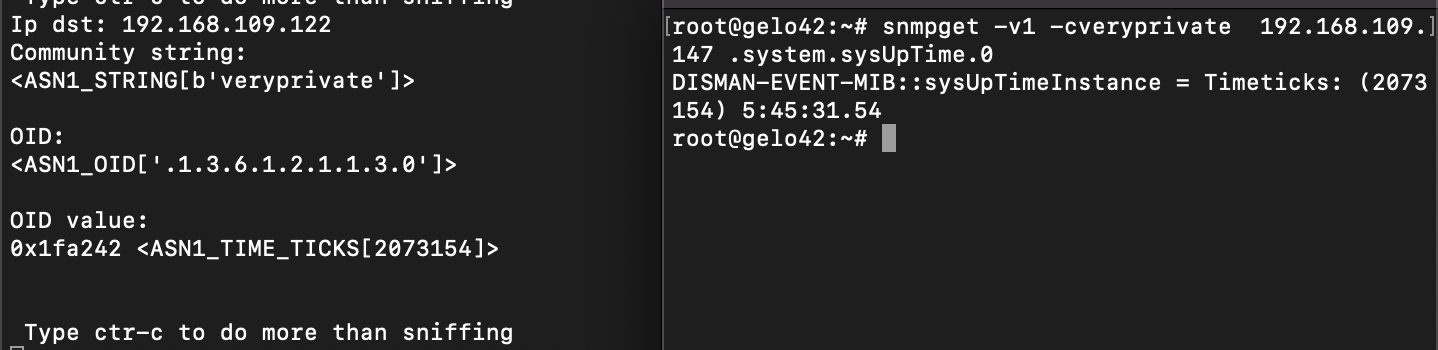
\includegraphics[width=1\linewidth,keepaspectratio]{SNMPSniffing.png}
    \caption{SNMP passive attack}
    \label{fig:SNMPPassiveAttack}
\end{figure}
\FloatBarrier

\begin{figure}[h!]
    \centering
    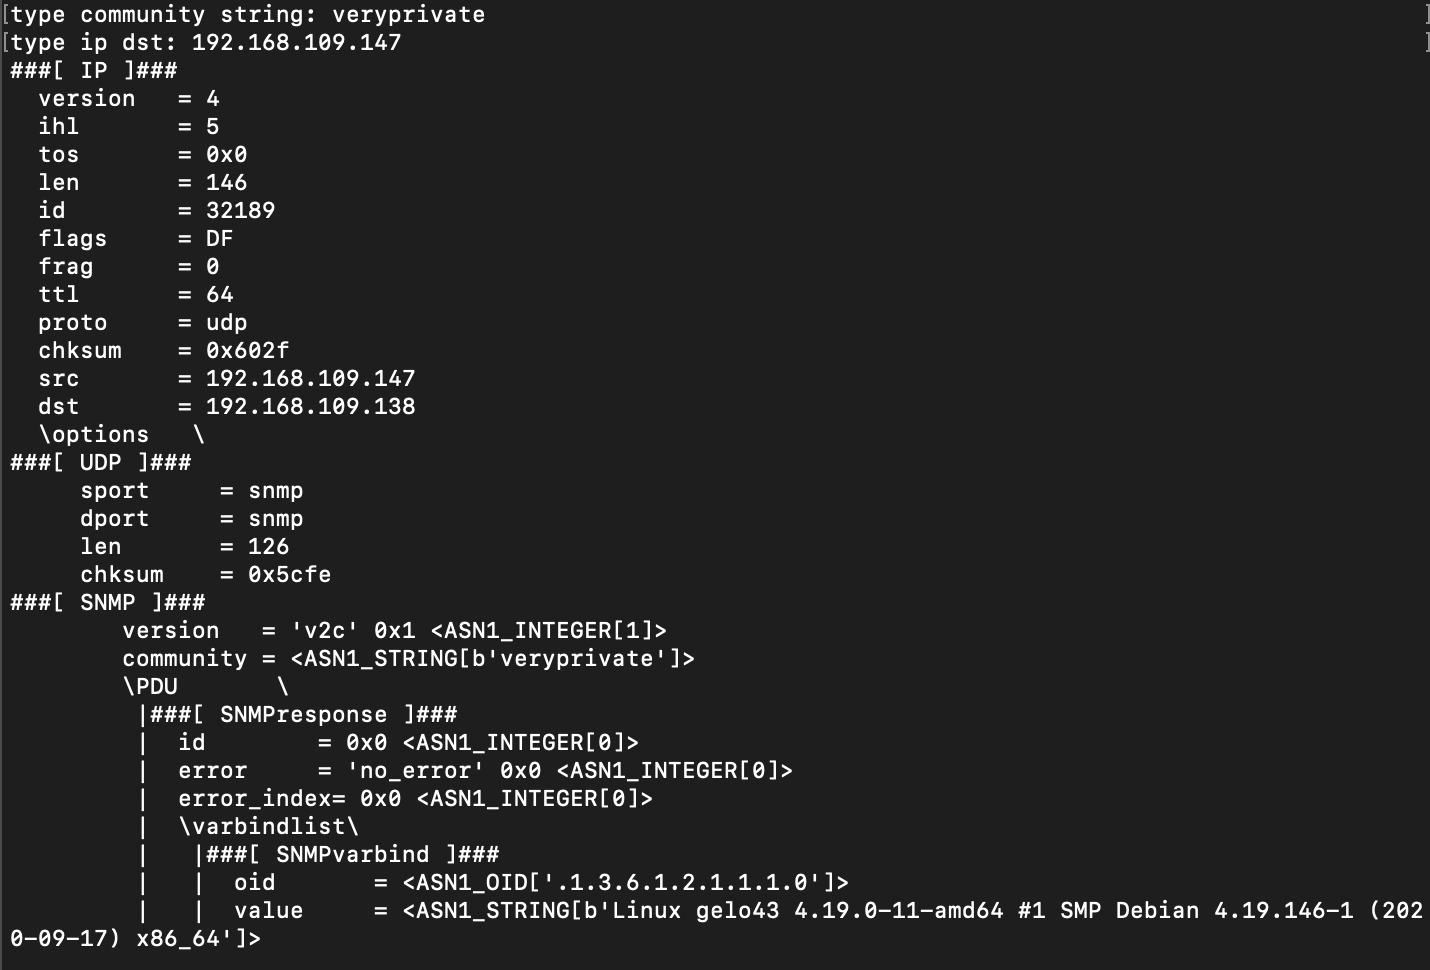
\includegraphics[width=1\linewidth,keepaspectratio]{SNMPAttack.png}
    \caption{SNMP active attack}
    \label{fig:SNMPActiveAttack}
\end{figure}
\FloatBarrier

In order to demonstrate both the passive and active Telnet attacks, the setup
present in \ref{fig:TelnetAttack} was implemented.
One VM was used as a legitimate client for the Telnet service while the 
attacker simultaneously intercepted and sniffed its connection - allowing the 
attacker to passively collect all the client's traffic.
After both victims were identified (Telnet's client and server), the attacker 
launches the mentioned reverse shell and waits for it on a running netcat 
instance - which can be seen in the right part of figure \ref{fig:TelnetAttack}.
Finally, the user's legitimate connection is shutdown due to the aforementioned 
RST forged packet sent by the attacker to the server.

\begin{figure}[h!]
    \centering
    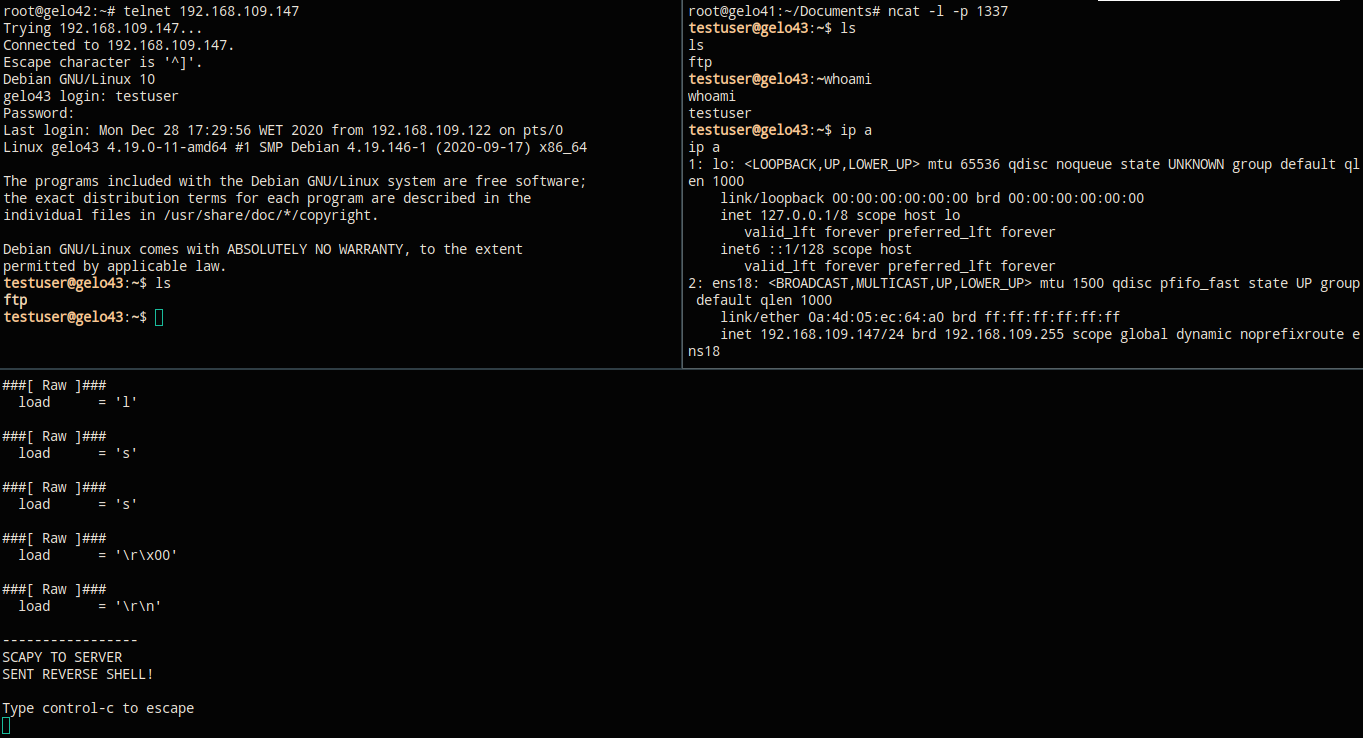
\includegraphics[width=1\linewidth,keepaspectratio]{ReverseShell.png}
    \caption{Telnet active attack - user in top-left, attacker reverse shell 
            in top-right, attacker Scapy bottom}
    \label{fig:TelnetAttack}
\end{figure}
\FloatBarrier


For the demonstration of the SMTP passive attack, one of the victims is \textit{telnetting} to the SMTP Postfix server located at \textit{192.168.109.147}. The victim sends a regular email to the server and, as shown left in figure \ref{fig:SMTPPassiveAttack}, the attacker has access to the user sending email, the receiver and the email body. 
\begin{figure}[h!]
    \centering
    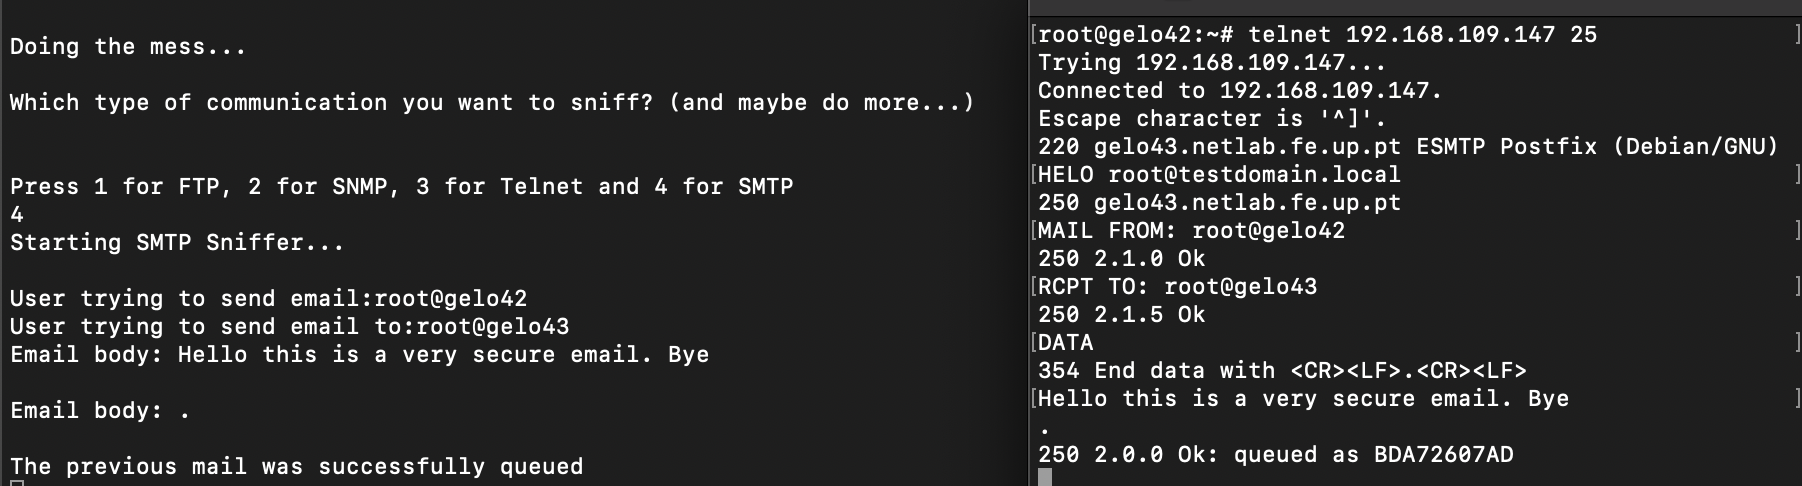
\includegraphics[width=1\linewidth,keepaspectratio]{SMTPAttack.png}
    \caption{SMTP passive attack}
    \label{fig:SMTPPassiveAttack}
\end{figure}
\FloatBarrier

Finally, the entire of the developed project can be found on our own personal
repositories at \url{https://github.com/RitaMartinho/SSRE}.
